\documentclass[a4paper]{article}
\usepackage{svg}
\usepackage{vntex}
\usepackage{pdflscape}
\usepackage{subcaption} % Thêm vào preamble của main.tex
\usepackage{rotating}
\usepackage{a4wide,amssymb,epsfig,latexsym,multicol,array,hhline,fancyhdr}
\usepackage{minted}
\usepackage{booktabs}
\usepackage{float}
\usepackage{longtable} % Cho bảng dài
\usepackage{placeins}
\usepackage{capt-of}
\usepackage{tabularx} % Cho bảng có cột co giãn
\usepackage{caption}
\usepackage{subcaption}
\usepackage{booktabs}
\usepackage{amsmath}
\usepackage{float}
\usepackage{lastpage} 
% \usepackage[lined,boxed,commentsnumbered]{algorithm2e}
\usepackage{enumerate}
\usepackage{color}
\usepackage{graphicx}					% Standard graphics package
\usepackage{array}
\usepackage{tabularx, caption}
\usepackage{multirow}
\usepackage[framemethod=tikz]{mdframed}% For highlighting paragraph backgrounds
\usepackage{multicol}
\usepackage{rotating}
\usepackage{graphics}
\usepackage{wrapfig}
\usepackage{geometry}
\usepackage{setspace}
\usepackage{epsfig}
\usepackage{tikz}
\usepackage{listings}
\usetikzlibrary{arrows,snakes,backgrounds}
\usepackage{hyperref}
\usepackage{minted}
\usepackage{indentfirst}
\usepackage{cases} 
\usepackage{listings}
\usepackage{algorithm}
\usepackage{algpseudocode}
% \usepackage[english]{babel}
\renewcommand{\baselinestretch}{1.5}
\usepackage{xcolor}
\usepackage[most]{tcolorbox}
\renewcommand{\figurename}{Hình}
\definecolor{termBG}{HTML}{0C1C23}
\definecolor{termWhite}{HTML}{F8F8F2}

\lstset{
    language=C++,
    basicstyle=\ttfamily\footnotesize,
    numbers=left,
    numberstyle=\tiny,
    stepnumber=1,
    numbersep=5pt,
    backgroundcolor=\color{gray!10},
    keywordstyle=\color{blue}\bfseries,
    commentstyle=\color{green!50!black},
    stringstyle=\color{red},
    frame=single,
    breaklines=true,
}

\usepackage[most]{tcolorbox}
\newtcbox{\code}{on line, 
    arc=2pt,                % Độ bo tròn góc
    colback=gray!20,        % Màu nền (xám nhạt)
    colframe=gray!20,       % Viền cùng màu nền
    boxrule=0pt,            % Không độ dày viền
    boxsep=0pt, left=2pt, right=2pt, top=2pt, bottom=2pt, % Khoảng cách đệm
    fontupper=\ttfamily     % Font chữ kiểu code
}

\newtcolorbox{softbox}{
    colback=black!3,        % Màu nền: Xám rất nhạt (3% đen)
    colframe=black!3,       % Màu viền: Trùng màu nền (để không thấy viền)
    arc=8pt,                % Độ bo tròn góc
    boxrule=0pt,            % Độ dày viền = 0
    left=10pt, right=10pt, top=8pt, bottom=8pt, % Khoảng cách lề bên trong
    fontupper=\itshape\color{black!80} % Font chữ: Nghiêng và màu xám đậm (80% đen)
}

\definecolor{codegreen}{rgb}{0,0.6,0}
\definecolor{codegray}{rgb}{0.5,0.5,0.5}
\definecolor{codepurple}{rgb}{0.58,0,0.82}
\definecolor{backcolour}{rgb}{0.95,0.95,0.92}

\definecolor{termBG}{HTML}{0C1C23}    % Màu nền xanh đen đậm
\definecolor{termRed}{HTML}{FF5555}   % Màu đỏ
\definecolor{termYellow}{HTML}{F1FA8C}% Màu vàng
\definecolor{termWhite}{HTML}{F8F8F2} % Màu chữ trắng sáng
\definecolor{termGray}{HTML}{A9B7C6}  % Màu xám nhạt (nếu cần)

\lstdefinestyle{terminalstyle}{
    basicstyle=\ttfamily\scriptsize\color{termWhite},
    backgroundcolor=\color{termBG},
    breaklines=true,
    columns=fullflexible,
    keepspaces=true,
    showstringspaces=false,
    frame=single,
    rulecolor=\color{termBG},
    framesep=4pt,
    numbers=none
}

% Lệnh tắt để tô màu cho nhanh
\newcommand{\cred}[1]{\textcolor{termRed}{#1}}
\newcommand{\cyellow}[1]{\textcolor{termYellow}{#1}}

% Cấu hình style cho C++
\lstdefinestyle{mystyle}{
    backgroundcolor=\color{backcolour},   
    commentstyle=\color{codegreen},
    keywordstyle=\color{magenta},
    numberstyle=\tiny\color{codegray},
    stringstyle=\color{codepurple},
    basicstyle=\ttfamily\footnotesize, % Font chữ kiểu máy đánh chữ, kích thước nhỏ
    breakatwhitespace=false,         
    breaklines=true,                 % Tự động xuống dòng nếu quá dài
    captionpos=b,                    
    keepspaces=true,                 
    numbers=left,                    % Hiển thị số dòng bên trái
    numbersep=5pt,                  
    showspaces=false,                
    showstringspaces=false,
    showtabs=false,                  
    tabsize=2,                       % Độ rộng tab = 2 spaces
    language=C++                     % Ngôn ngữ C++
}

\lstset{style=mystyle}

\usepackage{hyperref}
\hypersetup{
    colorlinks=true,
    linkcolor=black,      % Màu link nội bộ (mục lục, cross-reference)
    citecolor=red,        % ← Màu citation (references) - ĐỔI THÀNH ĐỎ
    urlcolor=blue,        % Màu URL
    filecolor=magenta     % Màu link file
}

%%%%%%%%
\usepackage{longtable}
\usepackage[shortlabels]{enumitem}

\setlength{\headheight}{40pt}
\pagestyle{fancy}
\fancyhead{} % clear all header fields
\fancyhead[L]{
 \begin{tabular}{rl}
    \begin{picture}(25,15)(0,0)
    \put(0,-8){
\includegraphics[width=8mm, height=8mm]{images/khtn.png}}
    \end{picture}&
	\begin{tabular}{l}
		\textbf{\bf \ttfamily Ho Chi Minh University of Science - VNUHCM}\\
		\textbf{\bf \ttfamily Faculty of Information Technology}
	\end{tabular}  	
 \end{tabular}
}
\fancyhead[R]{
	\begin{tabular}{l}
		\tiny \bf \\
		\tiny \bf 
	\end{tabular}  }
\fancyfoot{} % clear all footer fields
\fancyfoot[L]{\scriptsize \ttfamily Computer Network}
\fancyfoot[R]{\scriptsize \ttfamily Page {\thepage}}
\renewcommand{\headrulewidth}{0.3pt}
\renewcommand{\footrulewidth}{0.3pt}


%%%
\setcounter{secnumdepth}{4}
\setcounter{tocdepth}{3}
\makeatletter
\newcounter {subsubsubsection}[subsubsection]
\renewcommand\thesubsubsubsection{\thesubsubsection .\@alph\c@subsubsubsection}
\newcommand\subsubsubsection{\@startsection{subsubsubsection}{4}{\z@}%
                                    {-3.25ex\@plus -1ex \@minus -.2ex}%
                                    {1.5ex \@plus .2ex}%
                                    {\normalfont\normalsize\bfseries}}
\newcommand*\l@subsubsubsection{\@dottedtocline{3}{10.0em}{4.1em}}
\newcommand*{\subsubsubsectionmark}[1]{}
\makeatother

\definecolor{dkgreen}{rgb}{0,0.6,0}
\definecolor{gray}{rgb}{0.5,0.5,0.5}
\definecolor{mauve}{rgb}{0.58,0,0.82}

\lstset{frame=tb,
	language=Matlab,
	aboveskip=3mm,
	belowskip=3mm,
	showstringspaces=false,
	columns=flexible,
	basicstyle={\small\ttfamily},
	numbers=none,
	numberstyle=\tiny\color{gray},
	keywordstyle=\color{blue},
	commentstyle=\color{dkgreen},
	stringstyle=\color{mauve},
	breaklines=true,
	breakatwhitespace=true,
	tabsize=3,
	numbers=left,
	stepnumber=1,
	numbersep=1pt,    
	firstnumber=1,
	numberfirstline=true
}

\begin{document}

\begin{titlepage}
\begin{center}
VIETNAM NATIONAL UNIVERSITY HO CHI MINH CITY\\
HO CHI MINH CITY UNIVERSITY OF SCIENCE \\
FACULTY OF INFORMATION TECHNOLOGY
\end{center}

\vspace{0.7cm}

\begin{figure}[h!]
\begin{center}

\includegraphics[width=5cm]{images/khtn.png}
\end{center}
\end{figure}

\vspace{0.5cm}


\begin{center}
\begin{tabular}{c}
\multicolumn{1}{c}{\textbf{{\normalsize DEPARTMENT OF COMPUTER NETWORKS AND TELECOMMUNICATION}}}\\
~~\\
\hline
\\
\multicolumn{1}{c}{\textbf{{\Large REPORT OF PROJECT}}}\\  % ← Đổi từ {l} thành {c}
\\
\textbf{{\Large Project: Video Streaming System using RTSP/RTP protocols}}\\
\\
\hline
\end{tabular}
\end{center}

\vspace{0.5cm}

\begin{table}[h]
\begin{tabular}{rrll}
\hspace{4.5cm} & \textbf{Lecture:} & Lê Hà Minh\\
\hspace{4.5cm} & \textbf{Leader:} & Khang Phuc Nguyen & 24120068\\
\hspace{4.5cm} & Members: & Nghia Trong Hoang & 24120103\\
\hspace{4.5cm} &  & Trong Minh Pham & 24120151
\end{tabular}
\end{table}

\vspace{2.5cm}

\begin{center} {\footnotesize Ho Chi Minh City, 12/2025}
\end{center}
\end{titlepage}
%\thispagestyle{empty}


\thispagestyle{empty}

\newpage
\renewcommand{\contentsname}{Table of Contents}
\renewcommand{\tablename}{Table}
\renewcommand{\figurename}{Figure}
\renewcommand{\refname}{References}
\renewcommand{\listfigurename}{List of Figures}
\renewcommand{\listtablename}{List of Tables}

\tableofcontents

\newpage

\renewcommand{\arraystretch}{1.3} % Adjust row height
\setcounter{page}{1}

\section*{Giới thiệu}
Với sự phát triển của công nghệ số và nhu cầu giải trí của con người tăng cao, đặc biệt khi cuộc cách mạng 4.0, sự bùng nổ của Internet thì vai trò của Mạng Máy Tính trở nên ngày càng quan và có nhiều ứng dụng thực tiễn chẳng hạn là như là nhắn tin trực tuyến, làm việc trực tuyến và đặc biệt là trao đổi các thông tin, dữ liệu thông quan mạng. Đặc biệt trong số đó thì việc truyền các Video hoặc Ảnh thông qua được sử dụng ngày phổ biến trong các ứng dụng mạng xã hội như Facebook, TikTok và Youtube. 

Trong dự án này, nhóm đã tìm hiểu và thực hiện hóa một hệ thống đơn giản cho phép hai ứng dụng mạng có thể giao tiếp với nhau thông qua giao tiếp RTSP/RTP để có thể phát một video trực tuyến. Dự án này được làm với mục đích học tập và hiểu rõ hơn về các giao thức cũng như là cách hoạt động của các ứng dụng trong thực tế, mặt khác, dự án này cũng chỉ là mô phỏng lại cách phát trực tiếp một video giữa các ứng dụng nên được xây dựng không quá phức tạp và tối ưu.

Toàn bộ mã nguồn của dự án được xây dựng bằng ngôn ngữ \code{C++ 17}, sử dụng \code{CMake} để có thể build trên cả Window và Linux, cũng như là sử dụng các thư viện \code{winsock2} và \code{POSIX sockets} để tạo các socket cho việc giao tiếp giữa các ứng dụng. Bên cạnh đó, nhóm cũng đã áp dụng các kiến về \code{Design Pattern} cho dự án với mục đích là mã nguồn của dự án có thể tái sử dụng, sạch sẽ và dễ đọc, dễ sửa lỗi cũng như là tối ưu trong quá trình hoạt động.

Để có thể có mọt giao diện cho ứng dụng của bên phía \code{client} thì nhóm đã sử dụng \code{Qt6} để tạo ra một giao diện đơn giản và dễ sử dụng cho người dùng. Toàn bộ quá trình, giao thức, phản hồi và yêu cầu của \code{server} và \code{client} được dựa trên toàn bộ yêu cầu được đính kèm trong file \code{Socket\_2526} của thầy Lê Hà Minh \cite{lehaminh2024socket}. Nhóm xin chân thành cảm ơn thầy đã hỗ trợ và cung cấp tài liệu để nhóm có thể hoàn thành đồ án này một cách tốt đẹp nhất.

\begin{flushright}
\begin{minipage}{0.3\textwidth}
\centering 
\textbf{Nhóm Trưởng}\\
\textit{(Chữ ký và họ tên)}\\[0.5cm]
\textit{\large Khang}\\  
\textit{Nguyễn Phúc Khang}\\
\end{minipage}newpage
\hspace{1cm}
\end{flushright}
\vspace{2cm}
\begin{center} {\footnotesize Ho Chi Minh City, 12/2025}
\end{center}
\newpage
\section{Cơ sở lý thuyết}

Hệ thống truyền phát video trong đồ án được xây dựng dựa trên sự kết hợp chặt chẽ giữa kiến trúc mạng máy tính kinh điển và các kỹ thuật xử lý dữ liệu đa phương tiện thời gian thực, tuân thủ theo các yêu cầu của môn học \cite{lehaminh2024socket}. Phần này sẽ trình bày chi tiết về các giao thức, kỹ thuật socket nâng cao và các mẫu thiết kế phần mềm được áp dụng.

\subsection{Mô hình kiến trúc và Giao diện Socket}

Hệ thống vận hành dựa trên mô hình \textbf{Client-Server}, trong đó trách nhiệm được phân chia rõ ràng giữa hai thực thể. \textbf{Server} đóng vai trò là bên cung cấp dịch vụ thụ động (\textit{Passive Open}), chịu trách nhiệm lưu trữ tài nguyên video, quản lý các phiên làm việc và điều phối luồng dữ liệu. Ngược lại, \textbf{Client} đóng vai trò chủ động (\textit{Active Open}), khởi tạo các yêu cầu kết nối và thực hiện tái tạo hình ảnh từ dữ liệu nhận được.

Để hiện thực hóa cơ chế giao tiếp này, dự án sử dụng \textbf{Socket API} như một giao diện lập trình cốt lõi \cite{stevens2004unix}. Socket đóng vai trò là điểm cuối trong liên kết hai chiều giữa hai chương trình chạy trên mạng. Tùy thuộc vào yêu cầu về độ tin cậy hay tốc độ của từng loại dữ liệu, hệ thống sẽ khởi tạo loại socket phù hợp: \textbf{Stream Socket} (sử dụng TCP) cho kênh điều khiển nhằm đảm bảo tính chính xác tuyệt đối của lệnh, hoặc \textbf{Datagram Socket} (sử dụng UDP) cho kênh dữ liệu để tối ưu hóa độ trễ thời gian thực. Bên cạnh đó, các tùy chọn nâng cao như \texttt{SO\_REUSEADDR} cũng được áp dụng để quản lý trạng thái cổng kết nối hiệu quả, tránh các lỗi khóa tài nguyên thường gặp trong lập trình mạng UNIX \cite{stevens2004unix}.

\subsection{Các giao thức tầng giao vận}

Việc lựa chọn giao thức tầng giao vận là quyết định kỹ thuật quan trọng nhất ảnh hưởng đến hiệu năng của ứng dụng streaming. Thay vì chỉ sử dụng một giao thức đơn lẻ, hệ thống áp dụng cơ chế lai (Hybrid) để tận dụng ưu điểm của cả TCP và UDP theo kiến thức nền tảng về mạng máy tính \cite{kurose2021computer}. Sự khác biệt và phạm vi áp dụng của hai giao thức này trong dự án được tóm tắt tại Bảng \ref{tab:tcp_udp}.

\FloatBarrier
\begin{table}[H]
    \centering
    \caption{So sánh và phạm vi áp dụng của TCP và UDP trong hệ thống}
    \label{tab:tcp_udp}
    \begin{tabular}{p{0.15\textwidth}p{0.45\textwidth}p{0.3\textwidth}}
        \toprule
        \textbf{Giao thức} & \textbf{Đặc điểm kỹ thuật} & \textbf{Áp dụng trong dự án} \\
        \midrule
        \textbf{TCP} & Hướng kết nối, đảm bảo tin cậy, có kiểm soát luồng và tắc nghẽn, độ trễ cao hơn do cơ chế truyền lại (retransmission). & \textbf{Kênh RTSP:} Truyền tải các lệnh điều khiển quan trọng như \texttt{SETUP}, \texttt{PLAY}. \\
        \textbf{UDP} & Phi kết nối, không đảm bảo tin cậy, header nhỏ (8 byte), độ trễ thấp, hỗ trợ truyền thời gian thực. & \textbf{Kênh RTP:} Vận chuyển dữ liệu video (MJPEG). Chấp nhận mất gói để giữ độ trễ thấp. \\
        \bottomrule
    \end{tabular}
\end{table}
\FloatBarrier

\subsection{Giao thức điều khiển RTSP}

\textbf{Real-Time Streaming Protocol (RTSP)}, được định nghĩa trong RFC 2326 \cite{rfc2326}, hoạt động như một "bộ điều khiển từ xa" qua mạng cho các máy chủ đa phương tiện. Điểm khác biệt cốt lõi của RTSP so với HTTP là tính chất \textit{lưu trạng thái} (stateful). Server duy trì một phiên làm việc thông qua mã định danh \textbf{Session ID}, cho phép Server theo dõi trạng thái hiện tại của Client để phản hồi hợp lý. 

Quá trình chuyển đổi trạng thái của hệ thống tuân theo quy trình nghiêm ngặt: từ trạng thái \textbf{INIT} (khởi tạo), chuyển sang \textbf{READY} (sẵn sàng) sau khi thiết lập tài nguyên thành công, và cuối cùng là \textbf{PLAYING} (đang phát) khi luồng dữ liệu bắt đầu được truyền tải. Các phương thức điều khiển chính được mô tả trong Bảng \ref{tab:rtsp_methods}.

\FloatBarrier
\begin{table}[H]
    \centering
    \caption{Các phương thức RTSP và chức năng tương ứng}
    \label{tab:rtsp_methods}
    \begin{tabular}{p{0.2\textwidth}p{0.7\textwidth}}
        \toprule
        \textbf{Phương thức} & \textbf{Mô tả chức năng} \\
        \midrule
        \texttt{SETUP} & Khởi tạo phiên làm việc. Client gửi cổng nhận RTP (\textit{client\_port}), Server phản hồi với \textit{Session ID} và cổng truyền của Server. \\
        \texttt{PLAY} & Yêu cầu Server bắt đầu truyền dữ liệu RTP. Server chuyển trạng thái sang PLAYING. \\
        \texttt{PAUSE} & Tạm dừng luồng dữ liệu. Server ngừng gửi gói tin nhưng vẫn giữ nguyên phiên làm việc và trạng thái kết nối. \\
        \texttt{TEARDOWN} & Kết thúc phiên làm việc. Server đóng kết nối, giải phóng bộ đệm và thu hồi Session ID. \\
        \bottomrule
    \end{tabular}
\end{table}
\FloatBarrier

\subsection{Giao thức vận chuyển RTP và Cấu trúc gói tin}

Trong khi RTSP chịu trách nhiệm điều khiển, \textbf{Real-time Transport Protocol (RTP)} theo tiêu chuẩn RFC 3550 \cite{rfc3550} đảm nhiệm vai trò vận chuyển dữ liệu video thực tế. Do đặc thù của giao thức UDP là không đảm bảo thứ tự, RTP bổ sung một phần tiêu đề (Header) dài 12 byte vào trước mỗi gói dữ liệu để cung cấp thông tin tái đồng bộ.

Ba trường thông tin quan trọng nhất trong RTP Header bao gồm: \textbf{Sequence Number} (16 bit) giúp bên nhận phát hiện mất gói và sắp xếp lại các gói tin bị đảo lộn; \textbf{Timestamp} (32 bit) đóng vai trò nhãn thời gian để đồng bộ hóa tốc độ hiển thị khung hình, đảm bảo video không bị tua nhanh hoặc chậm bất thường; và \textbf{Marker Bit} (1 bit) dùng để đánh dấu gói tin cuối cùng của một khung hình, hỗ trợ quá trình tái lắp ráp dữ liệu phân mảnh.

\subsection{Kỹ thuật Video Streaming và Xử lý bộ đệm}

Để đảm bảo khả năng truyền tải video mượt mà trên môi trường mạng biến động, hệ thống áp dụng các kỹ thuật xử lý dữ liệu nâng cao liên quan đến định dạng nén, phân mảnh và cơ chế đệm.

\subsubsection{Định dạng MJPEG và Phân mảnh gói tin (Fragmentation)}
Dự án sử dụng chuẩn nén \textbf{MJPEG (Motion JPEG)}, nơi mỗi khung hình video là một bức ảnh JPEG độc lập sử dụng kỹ thuật nén nội khung (intra-frame compression) \cite{tekalp2015digital}. Phương pháp này tuân thủ RFC 2435 \cite{rfc2435} và mang lại khả năng chịu lỗi cao, vì việc mất một gói tin chỉ ảnh hưởng cục bộ đến khung hình hiện tại mà không gây lỗi dây chuyền cho các khung hình kế tiếp.

Tuy nhiên, kích thước của một khung hình video (đặc biệt ở độ phân giải HD) thường vượt quá giới hạn \textbf{MTU (Maximum Transmission Unit)} của mạng Ethernet (thông thường là 1500 byte). Để giải quyết vấn đề này, dự án áp dụng kỹ thuật \textbf{Phân mảnh cấp ứng dụng} (Application-Level Fragmentation). Một khung hình lớn sẽ được chia nhỏ thành nhiều gói RTP có kích thước tối đa 1400 byte. Hệ thống sử dụng mẫu thiết kế \textbf{Strategy Pattern} \cite{gamma1994design} để linh hoạt chuyển đổi thuật toán xử lý giữa video SD (có thể không cần phân mảnh) và video HD (bắt buộc phân mảnh), đảm bảo tính tương thích và hiệu năng cao nhất.

\subsubsection{Cơ chế Bộ đệm (Buffering) và Kiểm soát Jitter}
Hiện tượng \textbf{Jitter} (sự biến thiên độ trễ gói tin) là nguyên nhân chính gây ra tình trạng giật hình trong streaming \cite{kurose2021computer}. Để khắc phục, Client được thiết kế hoạt động theo mô hình \textbf{Producer-Consumer} với một \textbf{Frame Buffer} trung gian. Luồng nhận mạng đóng vai trò Producer, liên tục tái lắp ráp các gói tin RTP và đẩy khung hình hoàn chỉnh vào hàng đợi. Luồng hiển thị giao diện đóng vai trò Consumer, lấy khung hình ra để hiển thị theo định kỳ.

Đặc biệt, kỹ thuật \textbf{Pre-buffering} (Tiền tải) được áp dụng nhằm yêu cầu Client phải tích lũy đủ một lượng khung hình nhất định (ngưỡng $N$ frames) trước khi bắt đầu phát. Cơ chế này giúp tạo ra một vùng đệm an toàn, triệt tiêu các dao động tức thời của mạng và đảm bảo trải nghiệm xem video liên tục.

\subsection{Các mẫu thiết kế phần mềm (Design Patterns)}

Để đảm bảo mã nguồn có khả năng mở rộng, dễ bảo trì và tuân thủ các nguyên lý lập trình hướng đối tượng, dự án đã áp dụng một số mẫu thiết kế phần mềm kinh điển được đề xuất bởi Gamma và cộng sự \cite{gamma1994design}. Việc áp dụng các mẫu này giúp giải quyết các vấn đề phổ biến trong việc khởi tạo đối tượng, quản lý trạng thái toàn cục và đơn giản hóa các giao diện phức tạp.

\subsubsection{Mẫu thiết kế Builder (Builder Pattern)}
Trong giao thức RTP, việc khởi tạo một gói tin (\texttt{RTPPacket}) đòi hỏi thiết lập rất nhiều tham số chi tiết cho phần tiêu đề (Header) như: phiên bản (Version), chỉ số đếm (Sequence Number), nhãn thời gian (Timestamp), bit đánh dấu (Marker), và loại tải (Payload Type). Việc sử dụng một hàm khởi tạo (Constructor) với quá nhiều tham số sẽ khiến mã nguồn khó đọc và dễ gây lỗi.

Để giải quyết vấn đề này, dự án áp dụng mẫu thiết kế \textbf{Builder Pattern}. Cụ thể, lớp \texttt{RTPPacketBuilder} (nằm trong thư mục \texttt{common/src/rtp}) được xây dựng để tách biệt quá trình khởi tạo phức tạp khỏi biểu diễn của đối tượng. Mẫu thiết kế này cho phép thiết lập từng thuộc tính của gói tin một cách tuần tự và rõ ràng thông qua chuỗi các phương thức (method chaining) trước khi gọi phương thức \texttt{build()} để tạo ra đối tượng gói tin hoàn chỉnh.

\subsubsection{Mẫu thiết kế Singleton (Singleton Pattern)}
Trong một hệ thống phân tán, có những thành phần cần đảm bảo tính duy nhất và có thể truy cập toàn cục từ bất kỳ đâu trong chương trình, điển hình là bộ ghi nhật ký (Logger) và bộ quản lý cấu hình (Configuration Manager).

Dự án áp dụng mẫu thiết kế \textbf{Singleton Pattern} cho các lớp \texttt{Logger} và \texttt{Config} (trong thư mục \texttt{common/src/utils}). Mẫu thiết kế này đảm bảo rằng chỉ có duy nhất một thể hiện (instance) của lớp \texttt{Logger} được tạo ra trong suốt vòng đời ứng dụng, giúp đồng bộ hóa việc ghi log từ nhiều luồng (thread) khác nhau vào một tệp tin hoặc màn hình console duy nhất, tránh tình trạng xung đột tài nguyên. Tương tự, \texttt{Config} đóng vai trò là kho chứa thông tin cấu hình trung tâm (như địa chỉ IP, cổng, kích thước bộ đệm) mà mọi thành phần khác đều có thể truy xuất.

\subsubsection{Mẫu thiết kế Facade (Facade Pattern)}
Lập trình mạng trên hệ điều hành thường yêu cầu tương tác với các API cấp thấp phức tạp của thư viện Berkeley Sockets (như \texttt{sockaddr\_in}, \texttt{bind}, \texttt{listen}, \texttt{setsockopt}). Việc gọi trực tiếp các hàm C này rải rác trong mã nguồn sẽ làm giảm tính trừu tượng và khó chuyển đổi giữa các nền tảng (như Windows và Linux).

Để khắc phục, lớp \texttt{Socket} (trong thư mục \texttt{common/src/network}) được thiết kế như một \textbf{Facade} (mặt tiền). Lớp này cung cấp một giao diện lập trình hướng đối tượng đơn giản và thống nhất (với các phương thức như \texttt{send()}, \texttt{recv()}, \texttt{bind()}) để che giấu sự phức tạp của các lời gọi hệ thống bên dưới. Nhờ đó, các tầng cao hơn của ứng dụng (như RTSP Server hay RTP Sender) chỉ cần làm việc với đối tượng \texttt{Socket} mà không cần quan tâm đến chi tiết cài đặt của hệ điều hành.

\FloatBarrier
\begin{table}[H]
    \centering
    \caption{Tổng hợp các mẫu thiết kế được áp dụng trong cấu trúc mã nguồn}
    \label{tab:design_patterns}
    \begin{tabular}{p{0.2\textwidth}p{0.3\textwidth}p{0.4\textwidth}}
        \toprule
        \textbf{Mẫu thiết kế} & \textbf{Loại (Category)} & \textbf{Áp dụng thực tế trong dự án} \\
        \midrule
        \textbf{Builder} & Creational (Khởi tạo) & \texttt{RTPPacketBuilder}: Xây dựng gói tin RTP phức tạp từng bước một. \\
        \textbf{Singleton} & Creational (Khởi tạo) & \texttt{Logger}, \texttt{Config}: Quản lý tài nguyên duy nhất (log file, cấu hình) toàn cục. \\
        \textbf{Facade} & Structural (Cấu trúc) & \texttt{Socket}: Đóng gói và đơn giản hóa các thao tác với thư viện socket cấp thấp của hệ điều hành. \\
        \textbf{Strategy} & Behavioral (Hành vi) & \texttt{EncodingStrategy}: Linh hoạt thay đổi thuật toán phân mảnh cho video SD và HD (đã đề cập ở phần trước). \\
        \bottomrule
    \end{tabular}
\end{table}
\FloatBarrier

\subsection{Github Repository}
Dự án được lưu trữ trên Github tại địa chỉ \url{https://github.com/khang1108/rocketProgramming}. Nhóm đã có đẩy code lên và cũng như là tạo các bản \code{release} cho các nền tảng Windows, macOS và Linux.

\section{Tổng quan kiến trúc hoạt động}

\subsection{Sơ đồ triển khai hệ thống (Deployment Diagram)}

Hình \ref{fig:deployment} minh họa kiến trúc triển khai của hệ thống trên hai máy vật lý riêng biệt. Server chạy tiến trình \texttt{./server 8554}, lắng nghe các yêu cầu RTSP trên cổng TCP 8554. Client chạy tiến trình \texttt{./client}, kết nối đến Server để điều khiển phát video và nhận luồng dữ liệu RTP qua UDP. Mỗi thành phần trong sơ đồ đại diện cho một module chức năng cụ thể trong mã nguồn, từ việc xử lý giao thức RTSP, đọc và mã hóa video, đóng gói RTP, đến tái lắp ráp và hiển thị khung hình.

\begin{figure}[H]
\centering
\begin{tikzpicture}[
    node distance=0.8cm,
    machine/.style={draw, rectangle, minimum width=6cm, minimum height=10cm, thick},
    component/.style={draw, rectangle, minimum width=4.5cm, minimum height=1cm, fill=blue!10},
    arrow/.style={->, >=stealth, thick},
    label/.style={font=\small}
]

% Machine 1 - Server
\node[machine] (server_machine) at (0,0) {};
\node[above=0.1cm of server_machine.north, font=\bfseries] {Machine 1 (Server)};
\node[below=0.05cm of server_machine.north, font=\small\ttfamily] {./server 8554};

% Server components
\node[component] (rtsp_server) at (0, 3.5) {RTSPServer};
\node[below=0.1cm of rtsp_server.south, font=\scriptsize] {(TCP:8554)};

\node[component] (video_stream) at (0, 1.8) {VideoStream};
\node[below=0.1cm of video_stream.south, font=\scriptsize] {(Read MJPEG)};

\node[component] (encoding_ctx) at (0, 0.1) {EncodingCtx};
\node[below=0.1cm of encoding_ctx.south, font=\scriptsize] {(Strategy)};

\node[component] (rtp_builder) at (0, -1.6) {RTPPacketBuilder};
\node[below=0.1cm of rtp_builder.south, font=\scriptsize] {(Builder)};

\node[component] (udp_socket_server) at (0, -3.3) {UDP Socket};
\node[below=0.1cm of udp_socket_server.south, font=\scriptsize] {(Send packets)};

% Arrows between server components
\draw[arrow] (rtsp_server) -- (video_stream);
\draw[arrow] (video_stream) -- (encoding_ctx);
\draw[arrow] (encoding_ctx) -- (rtp_builder);
\draw[arrow] (rtp_builder) -- (udp_socket_server);

% Machine 2 - Client
\node[machine] (client_machine) at (10,0) {};
\node[above=0.1cm of client_machine.north, font=\bfseries] {Machine 2 (Client)};
\node[below=0.05cm of client_machine.north, font=\small\ttfamily] {./client ...};

% Client components
\node[component] (rtsp_client) at (10, 3.5) {RTSPClient};
\node[below=0.1cm of rtsp_client.south, font=\scriptsize] {(State Pattern)};

\node[component] (frame_buffer) at (10, 1.8) {FrameBuffer};
\node[below=0.1cm of frame_buffer.south, font=\scriptsize] {(Observer)};

\node[component] (frame_display) at (10, 0.1) {FrameDisplay};
\node[below=0.1cm of frame_display.south, font=\scriptsize] {(UI)};

\node[component] (frame_reassembler) at (10, -1.6) {FrameReassembler};

\node[component] (rtp_receiver) at (10, -3.3) {RTPReceiver};
\node[below=0.1cm of rtp_receiver.south, font=\scriptsize] {(UDP:25000)};

% Arrows between client components
\draw[arrow] (rtsp_client) -- (frame_buffer);
\draw[arrow] (frame_buffer) -- (frame_display);
\draw[arrow] (frame_reassembler) -- (frame_display);
\draw[arrow] (rtp_receiver) -- (frame_reassembler);

% Communication between machines
\draw[<->, thick, red] (rtsp_server.east) -- (rtsp_client.west) node[midway, above, font=\small] {RTSP (TCP)};
\draw[->, ultra thick, green!60!black] (udp_socket_server.east) -- (rtp_receiver.west) node[midway, above, font=\small] {RTP (UDP)};

\end{tikzpicture}
\caption{Sơ đồ triển khai hệ thống video streaming phân tán}
\label{fig:deployment}
\end{figure}

\subsection{Định dạng thông điệp RTSP (RTSP Message Format)}

Giao thức RTSP sử dụng cú pháp văn bản dạng ASCII, tương tự HTTP, để dễ dàng đọc và gỡ lỗi. Mỗi thông điệp RTSP bao gồm một dòng bắt đầu (Request Line hoặc Status Line), các dòng tiêu đề (Headers), và một dòng trống (\texttt{\textbackslash r\textbackslash n}) để đánh dấu kết thúc thông điệp.

\subsubsection{Định dạng RTSP Request}
Một yêu cầu RTSP từ Client gửi đến Server có cấu trúc như sau (xem Hình \ref{fig:rtsp_request}):

\begin{figure}[H]
\centering
\begin{tikzpicture}[
    msgbox/.style={draw, rectangle, minimum width=9cm, minimum height=0.8cm, fill=yellow!10, font=\ttfamily\small, anchor=west},
    annotation/.style={font=\small\itshape, red!70!black}
]

% Draw message box
\draw[thick] (0,0) rectangle (10,3.5);

% Content lines
\node[msgbox] (line1) at (0.2, 2.9) {METHOD FILE RTSP/1.0\textbackslash r\textbackslash n};
\node[annotation, right=0.2cm of line1.east, anchor=west] {$\leftarrow$ Request line};

\node[msgbox] (line2) at (0.2, 2.0) {CSeq: <sequence\_number>\textbackslash r\textbackslash n};
\node[annotation, right=0.2cm of line2.east, anchor=west] {$\leftarrow$ Mandatory header};

\node[msgbox] (line3) at (0.2, 1.1) {[Additional headers]\textbackslash r\textbackslash n};
\node[annotation, right=0.2cm of line3.east, anchor=west] {$\leftarrow$ Optional headers};

\node[msgbox] (line4) at (0.2, 0.2) {\textbackslash r\textbackslash n};
\node[annotation, right=0.2cm of line4.east, anchor=west] {$\leftarrow$ Empty line (end)};

\end{tikzpicture}
\caption{Cấu trúc thông điệp RTSP Request}
\label{fig:rtsp_request}
\end{figure}

Trong đó:
\begin{itemize}
    \item \textbf{METHOD}: Phương thức điều khiển (ví dụ: \texttt{SETUP}, \texttt{PLAY}, \texttt{PAUSE}, \texttt{TEARDOWN})
    \item \textbf{FILE}: Đường dẫn đến tài nguyên video trên Server (ví dụ: \texttt{movie.mjpeg})
    \item \textbf{RTSP/1.0}: Phiên bản giao thức
    \item \textbf{CSeq}: Số thứ tự yêu cầu (bắt buộc), dùng để đối chiếu với phản hồi
    \item \textbf{Additional headers}: Các tiêu đề tùy chọn khác như \texttt{Session}, \texttt{Transport}
\end{itemize}

\subsubsection{Định dạng RTSP Response}
Server phản hồi lại Client với thông điệp có cấu trúc như Hình \ref{fig:rtsp_response}:

\begin{figure}[H]
\centering
\begin{tikzpicture}[
    msgbox/.style={draw, rectangle, minimum width=9cm, minimum height=0.8cm, fill=green!10, font=\ttfamily\small, anchor=west},
    annotation/.style={font=\small\itshape, blue!70!black}
]

% Draw message box
\draw[thick] (0,0) rectangle (10,3.5);

% Content lines
\node[msgbox] (line1) at (0.2, 2.9) {RTSP/1.0 <status\_code> <reason>\textbackslash r\textbackslash n};
\node[annotation, right=0.2cm of line1.east, anchor=west] {$\leftarrow$ Status line};

\node[msgbox] (line2) at (0.2, 2.0) {CSeq: <sequence\_number>\textbackslash r\textbackslash n};
\node[annotation, right=0.2cm of line2.east, anchor=west] {$\leftarrow$ Echo CSeq};

\node[msgbox] (line3) at (0.2, 1.1) {[Additional headers]\textbackslash r\textbackslash n};
\node[annotation, right=0.2cm of line3.east, anchor=west] {$\leftarrow$ Headers};

\node[msgbox] (line4) at (0.2, 0.2) {\textbackslash r\textbackslash n};
\node[annotation, right=0.2cm of line4.east, anchor=west] {$\leftarrow$ Empty line (end)};

\end{tikzpicture}
\caption{Cấu trúc thông điệp RTSP Response}
\label{fig:rtsp_response}
\end{figure}

\noindent
Trong đó:
\begin{itemize}
    \item \textbf{status\_code}: Mã trạng thái HTTP-like (ví dụ: \texttt{200} OK, \texttt{404} Not Found)
    \item \textbf{reason}: Chuỗi mô tả trạng thái (ví dụ: \texttt{OK}, \texttt{Not Found})
    \item \textbf{CSeq}: Phản chiếu lại số thứ tự từ yêu cầu để Client đối chiếu
    \item \textbf{Headers}: Các thông tin bổ sung như \texttt{Session}, \texttt{Transport}, \texttt{Content-Length}
\end{itemize}

Việc sử dụng \texttt{CSeq} (Command Sequence) trong cả Request và Response đảm bảo tính toàn vẹn của giao tiếp, đặc biệt trong môi trường mạng bất đồng bộ, giúp Client xác định chính xác phản hồi nào tương ứng với yêu cầu nào khi có nhiều yêu cầu được gửi đồng thời.

\subsection{Cấu trúc thư mục dự án (Project Folder Structure)}

Dự án được tổ chức theo mô hình module hóa rõ ràng, tách biệt giữa Server, Client và Common library. Hình \ref{fig:folder_structure} minh họa cấu trúc thư mục chi tiết của toàn bộ mã nguồn.

\begin{figure}[H]
\centering
\begin{lstlisting}[basicstyle=\ttfamily\small, frame=single, xleftmargin=1cm]
rocketProgramming/
|-- common/
|   |-- include/     (network, rtp, patterns, utils)
|   |-- src/         (Socket, Logger, Config)
|   `-- tests/       (test_rtsp_message, test_timer)
|
|-- server/
|   |-- include/     (network, rtp, video)
|   |-- src/         (RTSPServer, VideoStream, Encoding)
|   |-- config/      (server.conf)
|   `-- videos/      (*.Mjpeg files)
|
|-- client/
|   |-- include/     (ui, network, rtp, buffer)
|   `-- src/         (ClientUI, RTSPClient, RTPReceiver)
|
|-- setup/           (setup.py, setup.spec)
\end{lstlisting}
\caption{Cấu trúc thư mục dự án với phân chia module rõ ràng}
\label{fig:folder_structure}
\end{figure}

\textbf{Giải thích cấu trúc:}

\begin{itemize}
    \item \textbf{common/}: Thư viện dùng chung cho cả Server và Client
    \begin{itemize}
        \item \texttt{include/}: Header files tổ chức theo namespace (network, rtp, patterns, utils)
        \item \texttt{src/}: Implementation của Socket wrapper, RTP packet, Logger, Config manager
        \item \texttt{tests/}: Unit tests cho các thành phần cốt lõi (RTSP message parsing, Timer)
    \end{itemize}
    
    \item \textbf{server/}: Chương trình Server
    \begin{itemize}
        \item \texttt{include/network/}: RTSPServer, ServerWorker (multi-threading)
        \item \texttt{include/rtp/}: RTP sender, packet builder
        \item \texttt{include/video/}: VideoStream (MJPEG extraction), EncodingStrategy
        \item \texttt{src/}: Implementation tương ứng
        \item \texttt{config/}: File cấu hình server (port, video path, log level)
        \item \texttt{videos/}: Chứa các file video MJPEG để streaming
    \end{itemize}
    
    \item \textbf{client/}: Chương trình Client với Qt6 UI
    \begin{itemize}
        \item \texttt{include/ui/}: ClientUI, BufferedSlider (custom Qt widgets)
        \item \texttt{include/network/}: RTSPClient (state machine)
        \item \texttt{include/rtp/}: RTPReceiver, FrameReassembler
        \item \texttt{include/buffer/}: FrameBuffer (thread-safe queue, prebuffering)
        \item \texttt{src/}: Implementation tương ứng
    \end{itemize}
    
    \item \textbf{setup/}: Scripts tự động hóa build và deployment
    \begin{itemize}
        \item \texttt{setup.py}: Python script kiểm tra dependencies và build (cross-platform)
        \item \texttt{setup.spec}: PyInstaller spec để đóng gói
        \item \texttt{setup\_windows.bat}: Batch script cho Windows
    \end{itemize}
\end{itemize}

Cấu trúc này tuân theo nguyên tắc \textbf{separation of concerns}: mỗi module có trách nhiệm rõ ràng, header và source tách biệt, tests độc lập. Điều này giúp dễ dàng maintain, extend và test từng phần của hệ thống.

\section{Implementation}

Phần này đi sâu vào chi tiết hiện thực của từng module trong hệ thống, bao gồm tổ chức mã nguồn, phân tích các lớp chính, trích dẫn các đoạn mã quan trọng và giải thích lý do lựa chọn giải pháp kỹ thuật cụ thể.

\subsection{Tổ chức Codebase}
Dự án được tổ chức theo cấu trúc thư mục phân tách rõ ràng giữa Client, Server và các thành phần dùng chung (Common) để đảm bảo tính module hóa và dễ bảo trì.

\begin{itemize}
    \item \code{server/}: Chứa mã nguồn cho ứng dụng Server.
    \begin{itemize}
        \item \code{src/network/RTSPServer.cpp}: Lớp chính để lắng nghe kết nối TCP.
        \item \code{src/network/ServerWorker.cpp}: Lớp xử lý logic cho từng Client riêng biệt.
    \end{itemize}
    \item \code{client/}: Chứa mã nguồn cho ứng dụng Client.
    \begin{itemize}
        \item \code{src/ui/ClientUI.cpp}: Giao diện người dùng (Qt Framework).
        \item \code{src/network/RTSPClient.cpp}: Xử lý gửi/nhận tín hiệu RTSP.
    \end{itemize}
    \item \code{common/}: Chứa các thư viện dùng chung.
    \begin{itemize}
        \item \code{src/network/Socket.cpp}: Wrapper cho API Socket của hệ điều hành.
        \item \code{src/rtp/RTPPacket.cpp}: Logic đóng gói/giải gói dữ liệu RTP.
    \end{itemize}
\end{itemize}

\subsection{Server Implementation}

\subsubsection{Cơ chế đa luồng (Multi-threading)}
\textbf{Lý do thiết kế:} Server phải có khả năng phục vụ nhiều Client xem video cùng lúc. Nếu chỉ sử dụng một luồng duy nhất (Single-thread), khi Server đang gửi dữ liệu cho Client A, Client B sẽ phải chờ đợi, gây ra độ trễ lớn.

\textbf{Hiện thực:}
Trong \code{RTSPServer::run()}, chúng tôi sử dụng vòng lặp vô hạn để chấp nhận kết nối. Mỗi khi có kết nối mới, một \code{std::thread} mới được tạo ra để chạy \code{ServerWorker}.

\begin{lstlisting}[language=C++, caption={Vòng lặp chấp nhận kết nối trong RTSPServer.cpp}]
void RTSPServer::run() {
    running = true;
    while (running) {
        // Accept TCP connection from Client
        std::unique_ptr<Socket> clientSocket = listenSocket->accept();
        if (clientSocket) {
            int clientId = nextClientId++;
            // Create Worker to manage this Client
            auto worker = std::make_unique<ServerWorker>(clientId, std::move(clientSocket));
            
            // WHY: Create separate thread to avoid blocking main loop
            std::thread workerThread([w = worker.get()]() { w->run(); });
            workerThread.detach(); // Detach thread
            
            // Save session to list
            activeSessions.push_back({clientId, std::move(worker)});
        }
    }
}
\end{lstlisting}

\subsubsection{Xử lý yêu cầu RTSP (State Machine)}
\textbf{Lý do thiết kế:} Giao thức RTSP yêu cầu client và server phải đồng bộ về trạng thái (Ví dụ: Không thể gửi lệnh \code{PLAY} khi chưa \code{SETUP}). Sử dụng máy trạng thái (State Machine) giúp kiểm soát chặt chẽ luồng nghiệp vụ này.

\textbf{Hiện thực:}
Trong \code{ServerWorker::handleSetup}, ta kiểm tra trạng thái hiện tại phải là \code{INIT} mới cho phép chuyển sang \code{READY}.

\begin{lstlisting}[language=C++, caption={Kiểm tra trạng thái trong ServerWorker.cpp}]
std::string ServerWorker::handleSetup(const RTSPMessage::Request& request) {
    // WHY: Validate State to ensure correct workflow
    if (state_ != State::INIT)
        return RTSPMessage::buildResponse(400, "Invalid State", request.cseq);

    // ... Logic to open video file and get RTP port ...

    // Generate random Session ID
    sessionId_ = generateSessionId();
    state_ = State::READY; // State transition

    return RTSPMessage::buildResponse(200, "OK", request.cseq, 
        {{"Session", sessionId_}, {"Transport", "..."}});
}
\end{lstlisting}

\subsection{Client Implementation}

\subsubsection{Giao diện tương tác (ClientUI)}
\textbf{Lý do thiết kế:} Việc xử lý mạng (Network I/O) thường tốn thời gian và có thể block (treo) giao diện nếu chạy trên cùng một luồng UI. Tuy nhiên, với Qt Framework, ta có thể sử dụng cơ chế Signal/Slot bất đồng bộ để xử lý các sự kiện nút bấm một cách mượt mà.

\textbf{Hiện thực:}
Khi người dùng bấm nút \code{Setup}, hàm \code{onSetupClicked} được gọi. Nó thực hiện gửi yêu cầu xuống tầng mạng và cập nhật giao diện dựa trên kết quả trả về.

\begin{lstlisting}[language=C++, caption={Xử lý sự kiện Setup trong ClientUI.cpp}]
void ClientUI::onSetupClicked() {
    // Send SETUP command via RTSPClient object
    bool success = rtspClient_->sendSetup(videoFile_, clientRTPPort_);

    if (success) {
        state_ = State::READY;
        // WHY: Update button states (Enable/Disable) 
        // to prevent invalid user actions (e.g. clicking Play before Setup)
        updateButtonStates(); 
        
        // Enable timeline slider
        timelineSlider_->setEnabled(true);
    } else {
        Logger::getInstance().log(LogLevel::ERROR, "SETUP Failed");
    }
}
\end{lstlisting}

\subsubsection{Gửi yêu cầu RTSP}
Trong \code{RTSPClient}, các lệnh được đóng gói thành chuỗi ký tự theo đúng chuẩn RFC 2326. Việc xây dựng chuỗi thủ công giúp ta kiểm soát chính xác từng byte gửi đi.

\begin{lstlisting}[language=C++, caption={Tạo bản tin SETUP trong RTSPClient.cpp}]
bool RTSPClient::sendSetup(const std::string& videoFile, int clientRTPPort) {
    std::ostringstream req;
    // Build Request Line
    req << "SETUP " << videoFile << " RTSP/1.0\r\n";
    // Add required Headers
    req << "CSeq: " << ++cseq_ << "\r\n";
    req << "Transport: RTP/AVP/UDP;unicast;client_port=" << clientRTPPort << "-"
        << (clientRTPPort + 1) << "\r\n";
    req << "\r\n"; // End of Headers

    // Send via TCP Socket
    std::string resp = sendRtspRequest(req.str());
    
    // ... Parse response ...
}
\end{lstlisting}

\subsection{Data Protocol (RTP)}

\subsubsection{Đóng gói gói tin (Packetization)}
\textbf{Lý do thiết kế:} Dữ liệu video MJPEG rất lớn, không thể gửi nguyên một khung hình trong một gói UDP (vì giới hạn MTU). Ta cần sử dụng RTP (Real-time Transport Protocol) để chia nhỏ và đánh dấu thứ tự, giúp Client có thể ghép lại chính xác.

\textbf{Hiện thực:}
Lớp \code{RTPPacket} sử dụng các phép toán thao tác bit (Bitwise operations) để đóng gói các trường Header (Sequence Number, Timestamp, SSRC) vào mảng byte.

\begin{lstlisting}[language=C++, caption={Đóng gói RTP Header trong RTPPacket.cpp}]
void RTPPacket::encode() {
    // Byte 0: Version(2), Padding(1), Extension(1), CC(4)
    // WHY: Use Bitwise OR (|) and Shift (<<) to pack multiple fields into 1 byte
    header_[0] = (version_ << 6) | (padding_ << 5) | (extension_ << 4) | (cc_ & 0x0F);

    // Byte 1: Marker(1), PayloadType(7)
    header_[1] = (marker_ << 7) | (payloadType_ & 0x7F);

    // Byte 2,3: Sequence Number (16 bit)
    // Split into 2 bytes (Big-Endian / Network Byte Order)
    header_[2] = (sequenceNumber_ >> 8) & 0xFF;
    header_[3] = sequenceNumber_ & 0xFF;
    
    // ... Similar for Timestamp and SSRC ...
}
\end{lstlisting}

Cách làm này đảm bảo gói tin RTP tạo ra tương thích hoàn toàn với các phần mềm chuẩn (như VLC, Wireshark), đồng thời tối ưu hóa băng thông vì không gửi dư thừa bất kỳ byte nào.
\section{Results}

Phần này tổng hợp kết quả kiểm thử và xác nhận tính đúng đắn của các khối logic cốt lõi (RTSP message handling, Timer kiểm soát nhịp), đồng thời mô tả các hành vi runtime có thể quan sát được từ client UI và các thống kê có sẵn trong mã nguồn.

\subsection{Kết quả kiểm thử đơn vị (Unit Tests)}

Dự án cung cấp bộ kiểm thử trong \code{common/tests} cho hai thành phần có rủi ro lỗi cao: (1) xây dựng và phân tích RTSP message, (2) Timer điều phối thời gian. Các test được viết theo phong cách ``lightweight framework'' (assert + reporter) và có thể chạy độc lập với Qt.

\begin{table}[H]
\centering
\caption{Tổng hợp kết quả unit test ở tầng Common}
\label{tab:unit_tests}
\begin{tabular}{lrr}
\toprule
Test Suite & Số test & Kết quả \\
\midrule
\code{test\_rtsp\_message} & 15 & 15 passed, 0 failed \\
\code{test\_timer} & 13 & 13 passed, 0 failed \\
\bottomrule
\end{tabular}
\end{table}

Kết quả chạy test RTSPMessage thể hiện cả các kịch bản cơ bản lẫn round-trip (build rồi parse lại). Đoạn log dưới đây minh họa phần tổng kết của suite (trích nguyên văn từ output).

\begin{lstlisting}[language={}, caption={Output tổng kết của \texttt{test\_rtsp\_message}}, label={lst:rtsp_test_output}]
Total: 15 tests
Passed: 15
Failed: 0
\end{lstlisting}

Tương tự, Timer được kiểm tra với nhiều interval (25 FPS, 30 FPS, 60 FPS), kiểm tra drift (không sleep khi ``work time'' vượt interval), và stress test. Đoạn log tổng kết:

\begin{lstlisting}[language={}, caption={Output tổng kết của \texttt{test\_timer}}, label={lst:timer_test_output}]
Total: 13 tests
Passed: 13
Failed: 0
\end{lstlisting}

\subsection{Chỉ số runtime sẵn có ở Client}

Ngoài unit test, Client đã tích hợp các thống kê runtime cho RTP: số packet nhận, số packet ước lượng mất, tổng bytes, và phần trăm loss. Loss được tính bằng chênh lệch sequence; do đó thống kê phản ánh mất gói ``theo thứ tự'' (out-of-order có thể bị tính như lost nếu đến quá muộn hoặc bị bỏ qua ở Reassembler tùy kịch bản).

\begin{lstlisting}[language=C++, caption={Công thức phần trăm mất gói RTP}, label={lst:loss_formula}]
double RTPReceiver::getPacketLossPercentage() const {
    uint64_t total = packetReceived_ + packetLost_;
    if (total == 0) return 0.0;
    return (static_cast<double>(packetLost_) * 100.0) / static_cast<double>(total);
}
\end{lstlisting}

\subsection{Hành vi buffer và prebuffer quan sát từ UI}

UI triển khai hai cơ chế nhằm tối ưu trải nghiệm: (1) prebuffer trước khi phát, (2) điều chỉnh nhịp render theo mức buffer. Prebuffer được kích hoạt khi bắt đầu PLAY hoặc khi xảy ra ``rebuffering'' do buffer cạn; điều này làm tăng độ ổn định, đổi lại là tăng độ trễ đầu phát.

\begin{table}[H]
\centering
\caption{Các tham số buffer quan trọng và ý nghĩa vận hành}
\label{tab:buffer_params}
\begin{tabular}{lll}
\toprule
Tham số & Vị trí & Ý nghĩa \\
\midrule
\code{PREBUFFER\_FRAMES} & \code{ClientUI} & Số frame cần tích lũy trước khi bắt đầu render \\
\code{LOW\_BUFFER\_THRESHOLD} & \code{ClientUI} & Ngưỡng cảnh báo buffer thấp và tăng interval render \\
\code{MAX\_PAYLOAD\_SIZE} & \code{RTPPacket} & Giới hạn payload/packet để tránh IP fragmentation \\
\bottomrule
\end{tabular}
\end{table}

\begin{lstlisting}[language=C++, caption={UI chuyển sang trạng thái ``Buffering'' khi buffer chưa đủ}, label={lst:ui_buffering_state}]
statusLabel_->setText(QString("Buffering... %1/%2 frames (%3%)")
    .arg(bufferSize)
    .arg(PREBUFFER_FRAMES)
    .arg(percentage, 0, 'f', 1));
\end{lstlisting}

\subsection{Hướng dẫn triển khai và tái lập kết quả}

\subsubsection{Thiết lập dự án thông qua \code{setup.py}}

Để đơn giản hóa quy trình triển khai trên các nền tảng khác nhau, dự án cung cấp script tự động hóa \code{setup.py} thực hiện toàn bộ các bước từ kiểm tra phụ thuộc đến biên dịch mã nguồn.

\paragraph{Quy trình tự động}

Script \code{setup.py} được thiết kế để hoạt động trên Linux, Windows (MSYS2), và macOS. Khi chạy, script sẽ:

\paragraph*{Phát hiện hệ điều hành}: Sử dụng \code{platform.system()} để xác định môi trường thực thi
\textbf{Kiểm tra Qt6}: Tìm kiếm Qt6 qua các phương pháp:
    \begin{itemize}
        \item Kiểm tra \code{qmake6} trong PATH
        \item Thực hiện CMake find\_package
        \item Tìm kiếm trong đường dẫn cài đặt phổ biến (MSYS2 MinGW64, Homebrew, v.v.)
    \end{itemize}
\paragraph*{Hướng dẫn cài đặt Qt6}: Nếu không tìm thấy, hiển thị hướng dẫn chi tiết theo từng nền tảng
\paragraph*{Cấu hình CMake}: Tự động thiết lập \code{CMAKE\_PREFIX\_PATH} và generator phù hợp (Make/Ninja)
\paragraph*{Biên dịch song song}: Sử dụng \code{make -j} hoặc \code{ninja} với tất cả các lõi CPU
\paragraph*{Hiển thị hướng dẫn sử dụng}: In ra cú pháp chạy server/client với ví dụ cụ thể

\paragraph*{Cách sử dụng}
\noindent

\begin{lstlisting}[language=bash, caption={Chạy script setup tự động}, label={lst:setup_script}]
# Linux/macOS
python3 setup.py

# Windows (CMD/PowerShell)
python setup.py
\end{lstlisting}

\paragraph{Xử lý lỗi phổ biến}
\noindent
Script tích hợp xử lý các tình huống lỗi thường gặp:

\noindent
\small
\begin{tabular}{p{0.3\textwidth}p{0.65\textwidth}}
\toprule
\textbf{Lỗi} & \textbf{Xử lý tự động} \\
\midrule
Qt6 không tìm thấy & Hiển thị hướng dẫn cài đặt chi tiết theo nền tảng (MSYS2 cho Windows, apt/pacman cho Linux, Homebrew cho macOS) \\
CMake chưa cài đặt & Dừng và yêu cầu cài CMake với link tải \\
Không có quyền ghi thư mục & Gợi ý thay đổi quyền hoặc clone vào thư mục khác \\
Build thất bại & In đầy đủ stderr và gợi ý kiểm tra compiler/dependencies \\
\bottomrule
\end{tabular}

\vspace{0.5em}

\subsubsection{Chạy ứng dụng sau khi build}

Sau khi script hoàn tất, các file thực thi nằm trong thư mục \code{build/bin/}. Cú pháp dòng lệnh được thiết kế đơn giản và trực quan.

\paragraph{Khởi động Server}
\noindent
\begin{lstlisting}[language=bash, caption={Chạy server với port chỉ định}, label={lst:run_server}]
cd build/bin
./server <port>

# Example: Run on port 8554
./server 8554
\end{lstlisting}

Server sẽ lắng nghe kết nối RTSP trên port được chỉ định (mặc định 8554 theo chuẩn RTSP) và tự động bind UDP socket cho RTP.

\paragraph{Khởi động Client}
\noindent
\begin{lstlisting}[language=bash, caption={Chạy client với các tham số kết nối}, label={lst:run_client}]
cd build/bin
./client <server_ip> <port> <video_file>

# Example: Connect to local server
./client 127.0.0.1 8554 movie.Mjpeg

# Example: Connect to remote server
./client 192.168.1.100 8554 video.Mjpeg
\end{lstlisting}

Client sẽ hiển thị giao diện Qt6 với các nút điều khiển RTSP (SETUP, PLAY, PAUSE, TEARDOWN) và thanh timeline để tua video.

\subsubsection{Thu thập dữ liệu và log}

Trong quá trình chạy, hệ thống ghi log chi tiết vào:
\begin{itemize}
    \item \code{server.log}: Các sự kiện phía server (accept connection, session state, streaming loop)
    \item \code{client.log}: Các sự kiện phía client (RTSP response, RTP statistics, buffer state)
\end{itemize}

Client UI cũng hiển thị thống kê real-time: số packet nhận, số packet mất, tỷ lệ loss, buffer size, prebuffer progress, cho phép quan sát hành vi hệ thống mà không cần đọc log file.

\section{Giao diện của Client}
\FloatBarrier
\begin{figure}[H]
    \centering
    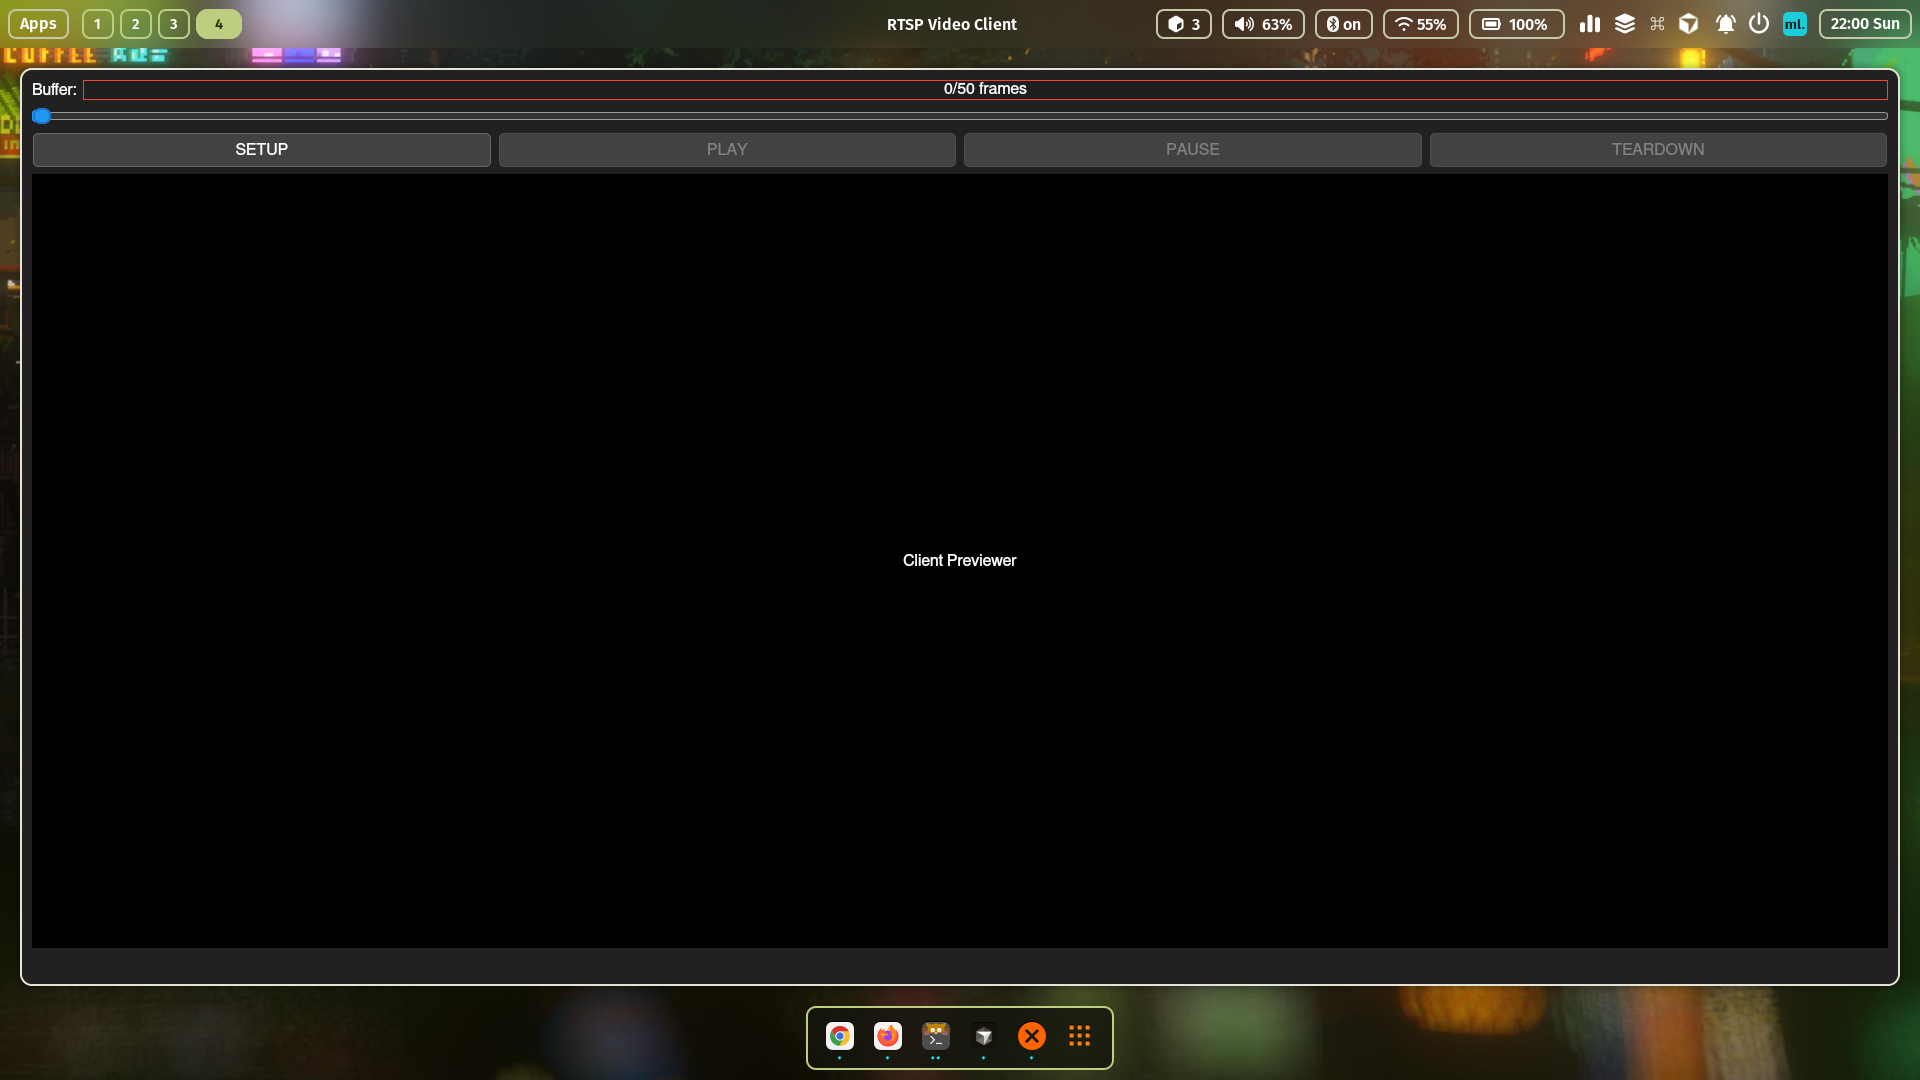
\includegraphics[width=0.9\textwidth]{images/client_ui_1.jpg}
    \caption{Giao diện của Client}
    \label{fig:client_ui}
\end{figure}

\begin{figure}[H]
    \centering
    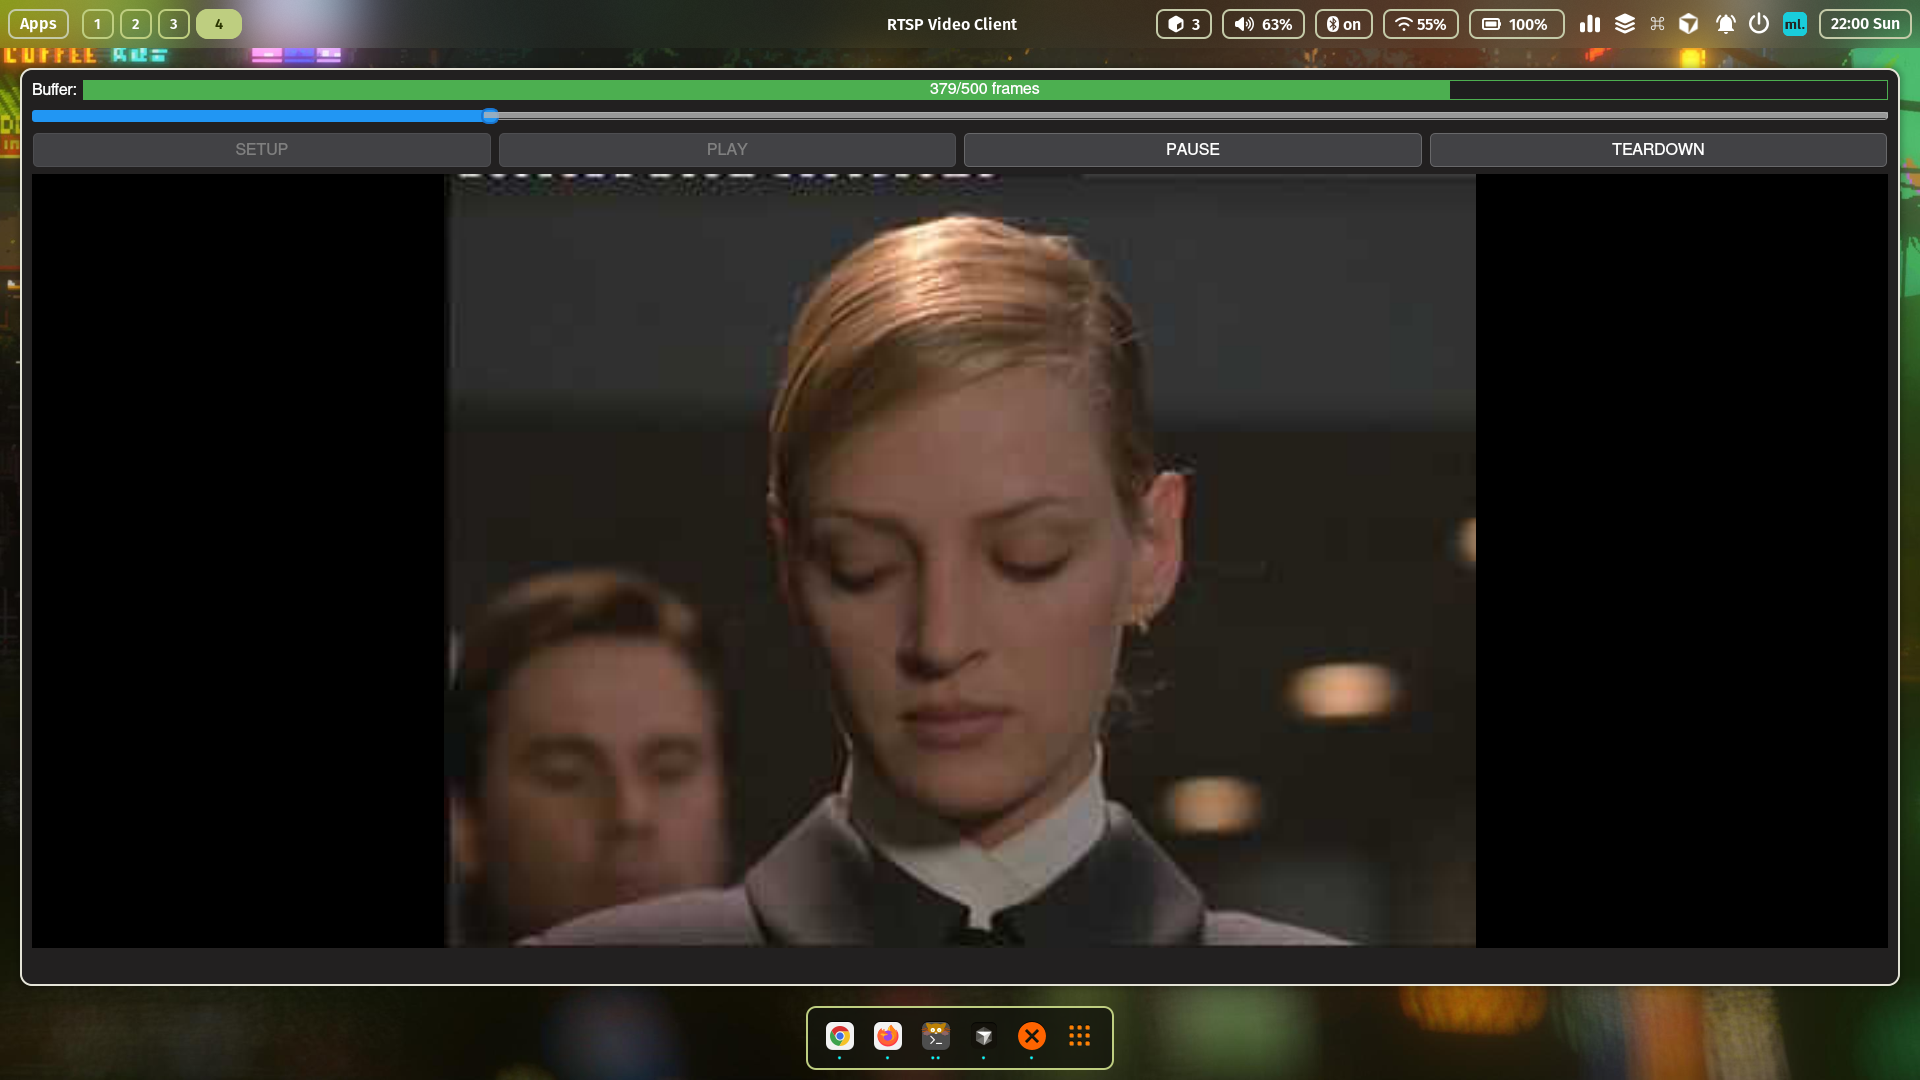
\includegraphics[width=0.9\textwidth]{images/client_ui_2.jpg}
    \caption{Giao diện của Client}
    \label{fig:client_ui}
\end{figure}

\section{Video Demo}
Dự án này được xây dựng có thể phù hợp với đa nền tảng khác nhau và đây là các video demo dự án từ đầu

\paragraph*{Windows}: Xem tại \url{https://youtu.be/yzEE6nu5VPk}

\paragraph*{Linux/MacOS}: Xem tại \url{https://youtu.be/vO6-jbP4yDU}
\section{Conclusion}

Hệ thống đã hiện thực đầy đủ một pipeline streaming video MJPEG theo mô hình RTSP (control plane, TCP) và RTP (data plane, UDP), với cấu trúc module hóa rõ ràng (Common/Server/Client), cơ chế đa luồng để phục vụ đồng thời nhiều client, và cơ chế buffer/prebuffer ở phía client để ổn định playback khi mạng jitter.

\subsection{Tổng kết đóng góp kỹ thuật theo mã nguồn}

Đóng góp cốt lõi của project không chỉ nằm ở việc ``chạy được streaming'', mà ở các quyết định hiện thực giúp hệ thống dễ bảo trì và mở rộng: chuẩn hóa RTSP ở \code{RTSPMessage}, chuẩn hóa networking ở \code{Socket}, áp dụng Builder cho RTP packet để kiểm soát tính hợp lệ, Strategy cho encode để tách SD/HD và phân mảnh.

\begin{lstlisting}[language=C++, caption={Tách biệt control plane và data plane: RTSP qua TCP, RTP qua UDP}, label={lst:control_data_plane}]
RTSPClient::connect()  -> Socket(TCP)::connect(serverIP, serverPort);
RTPReceiver::start()   -> Socket(UDP)::bind("0.0.0.0", clientRTPPort);
ServerWorker::handleSetup() -> parse Transport header (client_port=...)
ServerWorker::streamingLoop() -> Socket(UDP)::sendTo(..., clientIP, clientRTPPort);
\end{lstlisting}

Ngoài ra, lớp \code{FrameBuffer} có thể xem là một dạng ``video cache'' in-memory: nó lưu các frame đã ghép, tách biệt nhịp nhận (network-driven) khỏi nhịp phát (UI-driven). Đây là nền tảng để hiện thực prebuffer và các chính sách điều chỉnh nhịp phát theo mức buffer.

\begin{lstlisting}[language=C++, caption={Buffer như cache: producer (RTP) và consumer (UI) tách nhịp}, label={lst:buffer_cache}]
/* Producer thread */
frameReassembler_->frameBuffer()->push(frameData);

/* Consumer (UI timer) */
std::vector<uint8_t> frame;
if (frameBuffer_->tryPop(frame)) { render(frame); }
\end{lstlisting}

\subsection{Hạn chế hiện tại và đề xuất cải tiến dựa trên bằng chứng mã nguồn}

Một số điểm trong code hiện tại có thể ảnh hưởng độ ổn định hoặc độ chính xác timing; các đề xuất dưới đây được nêu dựa trực tiếp trên các đoạn mã hiện có.

\paragraph{(1) Tham số Timer ở Server chưa khớp mục tiêu 25 FPS.}
Trong \texttt{ServerWorker} có chú thích ``25 FPS (40ms)'' nhưng interval đang được khởi tạo là 10ms, dẫn tới nhịp gửi nhanh hơn dự kiến và có thể làm tăng tải CPU/network.

\begin{lstlisting}[language=C++, caption={Interval Timer ở ServerWorker đang đặt 10ms dù comment nói 40ms}, label={lst:timer_mismatch}]
// Initialize timer for 25 FPS (40ms)
frameTimer_ = std::make_unique<Timer>(10);
\end{lstlisting}

Khuyến nghị: đưa interval về 40ms hoặc đọc từ \code{Config} để đồng bộ với FPS mục tiêu và dễ hiệu chỉnh theo video.

\paragraph{(2) Logic \texttt{stop()} ở ServerWorker dùng \texttt{static} flag có thể gây lỗi khi có nhiều worker.}
Hàm \code{stop()} đang dùng \code{static std::atomic<bool> stopCalled} khiến chỉ worker đầu tiên được stop ``thực sự'', các worker còn lại sẽ return sớm. Đây là rủi ro rõ ràng nếu server phục vụ nhiều client đồng thời.

\begin{lstlisting}[language=C++, caption={Static stop flag có thể làm dừng sai khi nhiều worker}, label={lst:stop_static_bug}]
void ServerWorker::stop() {
    static std::atomic<bool> stopCalled{false};
    if (stopCalled.exchange(true)) {
        return;
    }
    // ...
}
\end{lstlisting}

Khuyến nghị: biến \code{stopCalled} thành member per-instance hoặc bỏ hoàn toàn (vì bản thân \code{running\_} và \code{streaming\_} đã là cờ dừng).

\paragraph{(3) Tính năng tua (seek) trên timeline hiện mới là thay đổi chỉ số hiển thị, chưa có RTSP Range.}
Client cập nhật \code{currentFrame\_} theo slider nhưng không gửi yêu cầu RTSP mới để server bắt đầu từ vị trí tương ứng; do đó ``seek'' hiện tại chỉ mang tính UI/telemetry.

\begin{lstlisting}[language=C++, caption={Seek hiện tại chỉ cập nhật currentFrame\_ ở UI}, label={lst:seek_ui_only}]
void ClientUI::onTimelineSliderReleased() {
    int targetFrame = timelineSlider_->value();
    currentFrame_ = targetFrame;
}
\end{lstlisting}

Khuyến nghị: mở rộng RTSP với header Range (NPT hoặc frame index), và server cần hỗ trợ reset \code{VideoStream} đến offset phù hợp (có thể bằng index table hoặc scan marker nhanh).

\paragraph{(4) Một số chi tiết định dạng RTSP request nên được chuẩn hóa tuyệt đối.}
Ví dụ, trong \code{RTSPClient::sendTeardown()} dòng request line thiếu khoảng trắng trước \code{RTSP/1.0}. Đây là lỗi định dạng có thể gây fail khi tương tác với server khác.

\begin{lstlisting}[language=C++, caption={Teardown request line thiếu khoảng trắng trước phiên bản}, label={lst:teardown_spacing}]
// Wrong:
ss << "TEARDOWN " << rtspUri_ << "RTSP/1.0\r\n";

// Correct:
ss << "TEARDOWN " << rtspUri_ << " RTSP/1.0\r\n";
\end{lstlisting}

Khuyến nghị: thống nhất tất cả request thông qua \code{RTSPMessage::buildRequest()} để loại bỏ sai sót format.

\subsection{Kết luận}

Với các thành phần đã hiện thực, dự án đáp ứng yêu cầu nền tảng của một hệ thống streaming RTSP/RTP có khả năng phân mảnh frame lớn, quản lý session, và buffer hóa ở client. Đồng thời, do code đã có cấu trúc pattern rõ ràng (Builder/Strategy/Singleton) và ranh giới module sạch, hệ thống sẵn sàng để mở rộng sang các tính năng ``production-grade'' hơn như Range seek, codec khác, adaptive bitrate, và cơ chế đồng bộ A/V trong các phiên bản tiếp theo.


\newpage
\listoffigures

\newpage
\listoftables

\newpage
\bibliographystyle{IEEEtran}
\bibliography{ref}
\end{document}